\documentclass[a4paper,11pt]{article}
\usepackage[margin=2cm]{geometry}
\usepackage{graphicx}
\usepackage{float}
\usepackage{amsmath}
\usepackage{xcolor}
\usepackage{listings}
\usepackage{comment}

\lstdefinestyle{matlab}{
	language=Matlab,
	basicstyle=\ttfamily\footnotesize,
	keywordstyle=\color{blue!70!black},
	commentstyle=\color{green!40!black},
	stringstyle=\color{purple!80!black},
	numbers=left, numberstyle=\tiny\color{gray}, numbersep=6pt,
	frame=single, rulecolor=\color{gray!60},
	breaklines=true, breakatwhitespace=false,
	columns=fullflexible, keepspaces=true,
	showstringspaces=false, tabsize=4,
	captionpos=t, aboveskip=8pt, belowskip=8pt
}

\lstdefinestyle{ccode}{
	language=C,
	morekeywords={int16_t, int32_t, uint16_t, uint32_t, __interrupt, volatile},
	basicstyle=\ttfamily\footnotesize,
	keywordstyle=\color{blue!70!black},
	commentstyle=\color{green!40!black},
	stringstyle=\color{purple!80!black},
	directivestyle=\color{orange!70!black},
	numbers=left, numberstyle=\tiny\color{gray}, numbersep=6pt,
	frame=single, rulecolor=\color{gray!60},
	breaklines=true, breakatwhitespace=false,
	columns=fullflexible, keepspaces=true,
	showstringspaces=false, tabsize=4,
	captionpos=t, aboveskip=8pt, belowskip=8pt
}

\title{ESP Lab1: Prep Sheet\\ \large Signal Modulation by Decimation and Interpolation}
\author{}
\date{}

\begin{document}
	\sloppy
	\maketitle
	
	\begin{table}[h]
		\centering
		\begin{tabular}{|l|l|l|}
			\hline
			\textbf{Group / Team} & \textbf{Team member 1:} & Pham, Tuong Minh \\
			\hline
			ESPL/01 / ? & \textbf{Team member 2:} & \\
			\hline
		\end{tabular}
	\end{table}
	
	
	
	\begin{table}[h]
		\centering
		\caption{Configuration of Labgroup 1}
		\small
		\begin{tabular}{|l|c|c|c|c|c|c|}
			\hline
			\textbf{Lab group} & \textbf{$M = L$} & \textbf{Chirp [kHz]} & \textbf{Length} & \textbf{$f_{bat}$} & \textbf{$f_s$ ADC, DAC} & \textbf{$x_\lambda$ at CH0 / CH1} \\
			\hline
			ESPL/01 & 3 & 18 \dots 21 & 2.5 s & 18 kHz & 50 kHz, 50 kHz & $\lambda=0$ / $\lambda=2$ \\
			\hline
		\end{tabular}
	\end{table}
	
	\setcounter{section}{2}
	\section{Preparation}
	
	\subsection*{Use of generative AI}
	
	Tool: Claude (Anthropic), October 2026. The lab instructions and the Moodle files were provided as context. Essential prompts (translated from German, condensed):
	\begin{enumerate}
		\item ``Write a prompt that I can use to work on the preparation tasks of ESP Lab 1.''
		\item ``Lab group ESPL/01: $M = L = 3$, chirp 18--21 kHz, 2.5 s, $f_{bat} = 18$ kHz,
		$f_s = 50$ kHz, polyphases $\lambda = 0$ / $\lambda = 2$. Create a commented MATLAB
		script for sections 3.1--3.5 with all required plots, using \texttt{firpmord}/\texttt{firpm}
		and \texttt{write\_coeff} as in the tutorial script. Explain for each section why the
		result is correct, using concrete frequencies. Extend \texttt{dec\_int\_standalone.c}
		to $M = L = 3$ and explain why \texttt{g\_PolyWUpdate} is necessary. Explain every
		non-trivial step so that I can explain the code in the lab.''
		\item "Create a Latex-textfile of the Word-Prepsheet-Template with Listing for Matlab code"
	\end{enumerate}
	
	
	% ------------------------------------------------------------------
	\subsection{Creating a Chirp Signal}
	
	\noindent\fbox{\parbox{\dimexpr\linewidth-2\fboxsep-2\fboxrule}{
			Add your results, including \textbf{Matlab code} and \textbf{figures}, to the preparation sheet.
			\textbf{Explain} why you think the result is correct.}}
	
	\medskip
	\newpage
	\begin{lstlisting}[style=matlab, caption={MATLAB code, parameters and Section 3.1}, label={lst:m31}]
		%% ESP Lab 1 - Preparation: Signal Modulation by Decimation and Interpolation
		% Lab group ESPL/01
		%   M = L = 3, chirp 18 ... 21 kHz, length 2.5 s, f_bat = 18 kHz
		%   fs (ADC, DAC) = 50 kHz, polyphases at DAC: CH0 -> lambda = 0, CH1 -> lambda = 2
		%
		% Requirements: Signal Processing Toolbox (chirp, spectrogram, firpmord, firpm, freqz)
		%               write_coeff.m (Moodle) in the same folder
		%
		% Run section by section (Ctrl+Enter) or the whole script (F5).
		
		clear; close all; clc;
		
		%% Parameters (Table 1, ESPL/01)
		fs     = 50e3;      % sampling frequency ADC and DAC [Hz]
		M      = 3;         % downsampling factor
		L      = 3;         % upsampling factor (M = L)
		f0     = 18e3;      % chirp start frequency [Hz]
		f1     = 21e3;      % chirp stop frequency [Hz]
		T      = 2.5;       % chirp length [s]
		f_bat  = 18e3;      % bat sound frequency [Hz]
		fs_low = fs/M;      % low sampling frequency f_s' = 16.667 kHz
		
		% identical spectrogram settings for all plots -> figures are comparable
		Nwin  = 1024;       % window length (Hamming)
		Nover = 768;        % overlap (75 %)
		Nfft  = 1024;       % FFT length
		
		% section for the stem plots: n = n1 ... n2 (60 samples, far from the start)
		n1 = 2000;
		n2 = 2059;
		
		%% 3.1 Chirp signal x[n]
		n = 0:round(T*fs)-1;            % sample index n = 0 ... 124999
		t = n/fs;                        % time axis [s]
		x = chirp(t, f0, T, f1);         % linear chirp, f(t) = f0 + (f1-f0)*t/T, amplitude 1
		
		figure('Name', '3.1 Chirp x[n]');
		subplot(2,1,1);
		spectrogram(x, hamming(Nwin), Nover, Nfft, fs, 'yaxis');
		title(sprintf('3.1  Spectrogram X[l,k]: chirp %g ... %g kHz, f_s = %g kHz', ...
		f0/1e3, f1/1e3, fs/1e3));
		
		subplot(2,1,2);
		sel = (n >= n1) & (n <= n2);     % logical index of the section
		stem(n(sel), x(sel), 'filled', 'MarkerSize', 3); grid on;
		xlabel('n'); ylabel('x[n]');
		title(sprintf('3.1 Time Domain Signal x[n] for n = %d ... %d ', n1, n2));
	\end{lstlisting}
	
	\begin{figure}[H]
		\centering
		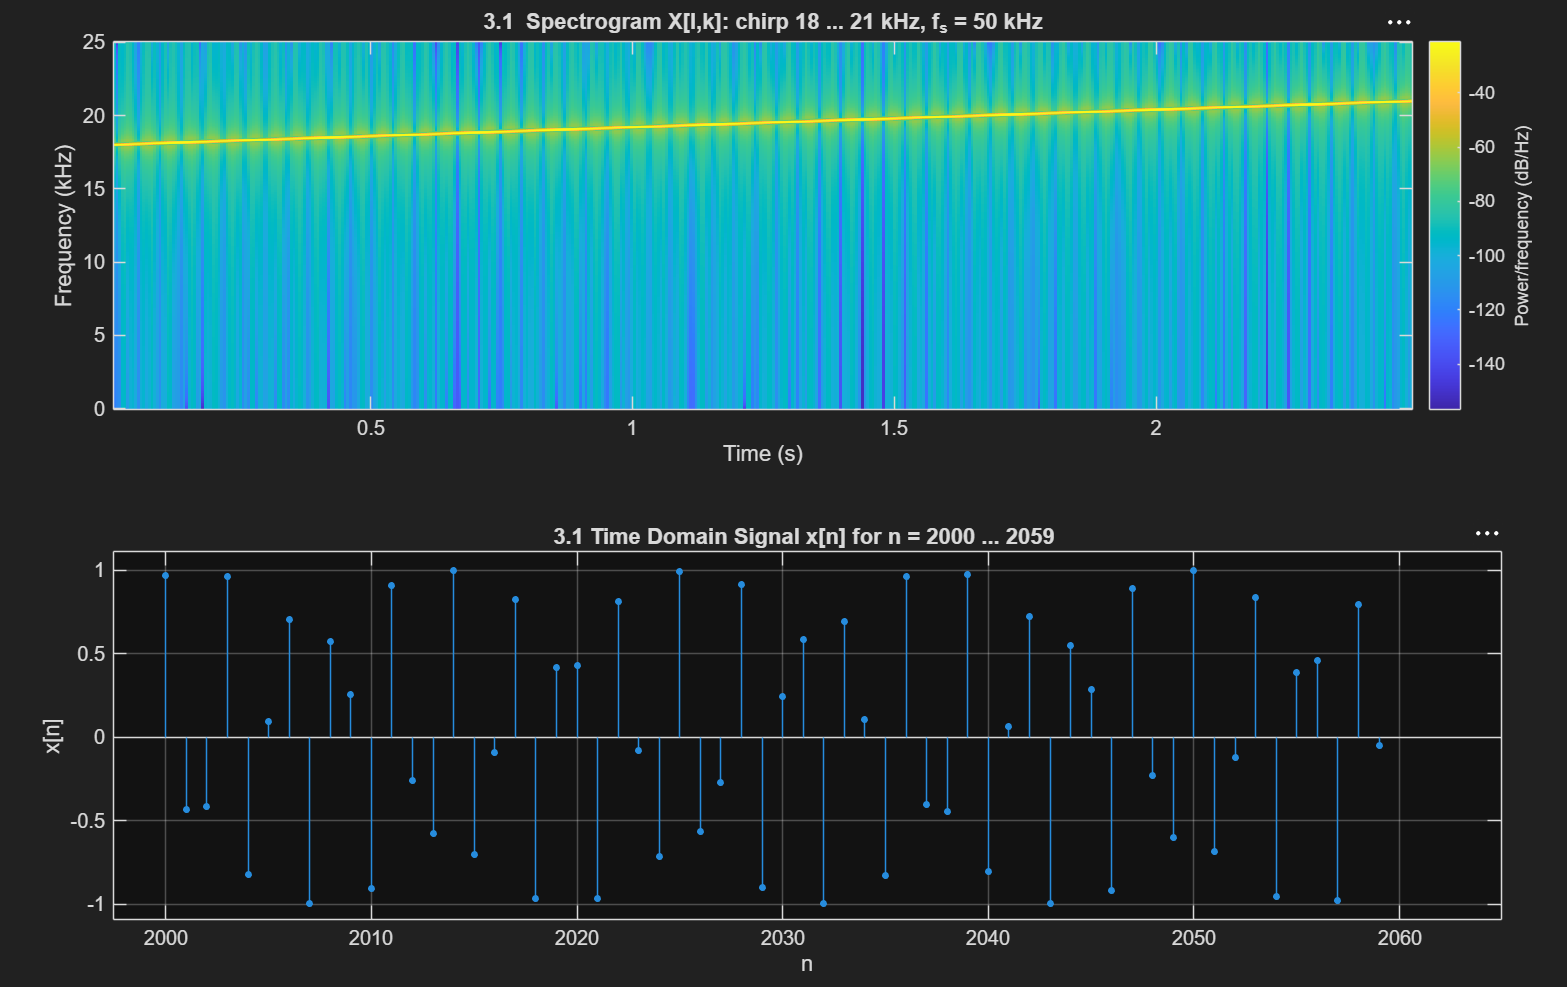
\includegraphics[width=\linewidth]{ESP1_3,1}
		\caption{Chirp signal $x[n]$: spectrogram $X[l,k]$ (top) and stem plot of the section $n = 2000, \dots, 2059$ (bottom).}
		\label{fig:esp131}
	\end{figure}
	
	
	
	
	\noindent\textbf{Explanation:} The chirp is generated on the time axis $t = n/f_s$ with \texttt{chirp(t, f0, T, f1)} (Listing~\ref{lst:m31}). The spectrogram in Fig.~\ref{fig:esp131} shows exactly this: a single straight line from 18\,kHz to 21\,kHz over 2.5\,s. %The background is not perfectly clean because each spectrogram segment is only a short window cut out of the signal. 
	This limitation in time spreads a small part of the signal energy over all frequencies (spectral leakage), far below the chirp itself. At n = 2000 the chirp frequency is about 18 kHz. With $f_s$ = 50 kHz there are fewer than three samples per period (50/18 $\approx$ 2.78), so the oscillation of the chirp cannot easily be recognised by the human eye. Instead, a low-frequency sine-like pattern is visible: every third sample lies on a slowly varying curve, because three samples correspond to slightly more than one full period of the chirp.
	
	
	% ------------------------------------------------------------------
	\subsection{Downsampling and Polyphase Representation}
	
	\noindent\fbox{\parbox{\dimexpr\linewidth-2\fboxsep-2\fboxrule}{
			Add your results, including \textbf{Matlab code} and \textbf{figures}, to the preparation sheet.
			\textbf{Explain} why you think the result is correct.}}
	
	\medskip
	
	\begin{lstlisting}[style=matlab, caption={MATLAB code, Section 3.2}, label={lst:m32}]
		%% 3.2 Downsampling by M and polyphase signals x_lambda[m] = x[m*M + lambda]
		Nshow = 100;                     % first 100 samples of each polyphase
		m     = 0:Nshow-1;               % low-rate index
		xpoly = cell(1, M);              % xpoly{lambda+1} = x_lambda[m]
		
		figure('Name', '3.2 Polyphase signals');
		for lambda = 0:M-1
		% MATLAB indices start at 1: index 1+lambda corresponds to n = lambda,
		% step M takes every M-th sample -> n = lambda, lambda+M, lambda+2M, ...
		xpoly{lambda+1} = x(1+lambda : M : end);
		
		subplot(M, 1, lambda+1);
		stem(m, xpoly{lambda+1}(1:Nshow), 'filled', 'MarkerSize', 3); grid on;
		ylabel(sprintf('x_{%d}[m]', lambda));
		title(sprintf('3.2  Polyphase \\lambda = %d:  x_{%d}[m] = x[%dm + %d],  f_s'' = %.3f kHz', ...
		lambda, lambda, M, lambda, fs_low/1e3));
		end
		
		
		% expected aliased frequency in the low-rate domain (fold into 0 ... fs'/2)
		falias = @(f) abs(f - round(f/fs_low)*fs_low);
		fprintf('3.2: chirp %g ... %g kHz appears at %.3f ... %.3f kHz after downsampling\n', ...
		f0/1e3, f1/1e3, falias(f0)/1e3, falias(f1)/1e3);
	\end{lstlisting}
	
	
	
	\begin{figure}[H]
		\centering
		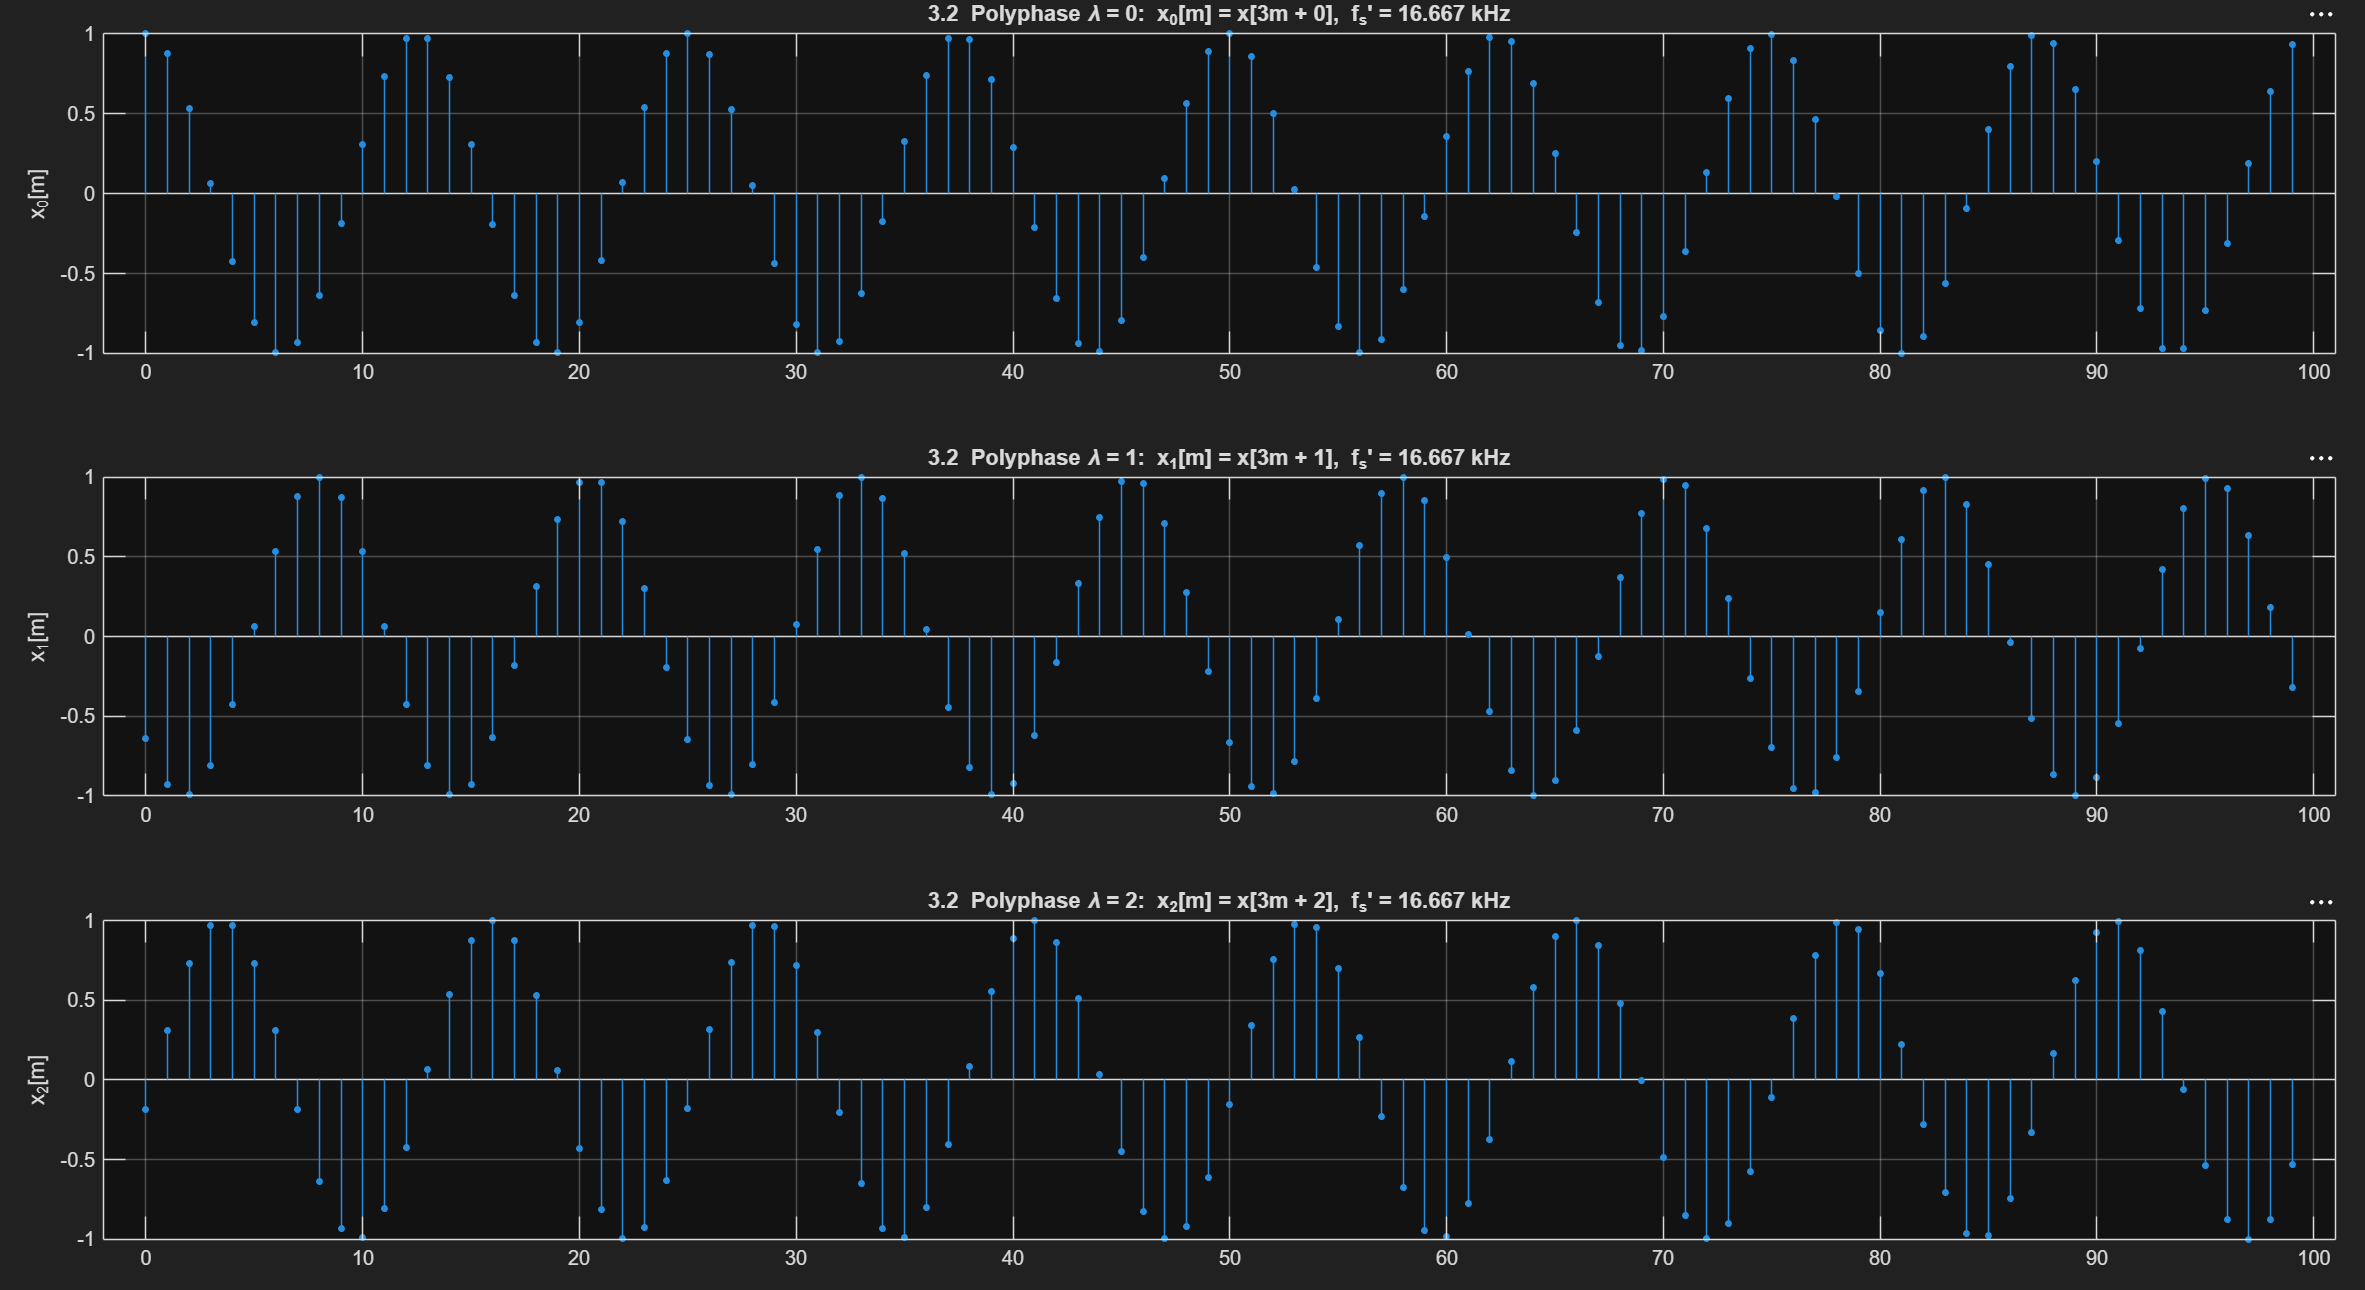
\includegraphics[width=\linewidth]{ESP1_3,2}
		\caption{Polyphase signals $x_\lambda[m] = x[3m + \lambda]$, $\lambda = 0, 1, 2$, first 100 samples at the low sampling frequency $f_s' = f_s/3 = 16.67$\,kHz.}
		\label{fig:esp132}
	\end{figure}
	
	\noindent\textbf{Explanation.} The three subplots in Fig.~\ref{fig:esp132} show the three downsampled signals (polyphases) $x_\lambda[m]$. Each polyphase takes every third sample of $x[n]$, starting at $n = \lambda$.
	
\begin{comment}
As discussed in the lecture, the polyphases are phase-shifted against each other: a delay of one sample at $f_s$ shifts the phase by
\[
\Delta\varphi = 360^\circ \cdot \frac{f}{f_s} = 360^\circ \cdot \frac{18\,\text{kHz}}{50\,\text{kHz}} \approx 130^\circ,
\]
so $x_1$ is shifted by about $130^\circ$ and $x_2$ by about $260^\circ$ relative to $x_0$. This can be checked at $m = 0$: $x_0[0] = \cos(0^\circ) = 1$, $x_1[0] = \cos(130^\circ) \approx -0.64$ and $x_2[0] = \cos(260^\circ) \approx -0.19$.
\end{comment}
	
	All three polyphases oscillate with the same low frequency of about 1.33\,kHz (about 12.5 samples per period). Since no anti-aliasing filter is applied, the chirp at 18\,kHz lies above $f_s'/2$ and is aliased to
	\[
	f' = f - f_s' = 18\,\text{kHz} - 16.67\,\text{kHz} \approx 1.33\,\text{kHz}.
	\]
	This is the slow pattern already visible in the stem plot of Section~3.1.
	
	\subsection{Upsampling without Interpolation Filter}
	
	\noindent\fbox{\parbox{\dimexpr\linewidth-2\fboxsep-2\fboxrule}{
			Add your results, including \textbf{Matlab code} and \textbf{figures}, to the preparation sheet.
			Explain the \textbf{shape of the spectrogram} and provide reasons \textbf{based on specific
				frequencies}. Assume that a \textbf{bat sound of $f_{bat}$} (as given in Table~1 for your ESPL
			group) is fed into the system's ADC. Is it \textbf{reproduced at the DAC output}? If so, at
			\textbf{what frequency} / frequencies?}}
	
	\medskip
	
	\begin{lstlisting}[style=matlab, caption={MATLAB code, Section 3.3}, label={lst:m33}]
		%% 3.3 Upsampling of x_0[m] by L WITHOUT interpolation filter
		x0 = xpoly{1};                       % polyphase lambda = 0
		yu = zeros(1, L*length(x0));         % y'[n] at high rate fs
		yu(1:L:end) = x0;                    % y'[nL] = x_0[n], L-1 zeros in between
		
		figure('Name', '3.3 Upsampler output y''[n]');
		subplot(2,1,1);
		spectrogram(yu, hamming(Nwin), Nover, Nfft, fs, 'yaxis');
		title(sprintf('3.3  Spectrogram Y''[l,k]: x_0[m] upsampled by L = %d, no interpolation filter', L));
		
		subplot(2,1,2);
		nu  = 0:length(yu)-1;
		sel = (nu >= n1) & (nu <= n2);
		stem(nu(sel), yu(sel), 'filled', 'MarkerSize', 3); grid on;
		xlabel('n'); ylabel('y''[n]');
		title(sprintf('3.3  y''[n] for n = %d ... %d  (every %d-th sample non-zero)', n1, n2, L));
		
		% where does a bat tone f_bat appear at the DAC output?
		fa    = falias(f_bat);                              % frequency in the low-rate domain
		f_img = [fa + (0:L-1)*fs_low, (1:L)*fs_low - fa];   % all images k*fs' +/- fa
		f_img = unique(f_img(f_img <= fs/2));               % only 0 ... fs/2 is visible
		fprintf('3.3: f_bat = %g kHz -> %.3f kHz after downsampling\n', f_bat/1e3, fa/1e3);
		fprintf('     upsampler output (0 ... %g kHz): %s kHz, each with amplitude 1/L = %.1f dB\n', ...
		fs/2e3, mat2str(round(f_img)/1e3), 20*log10(1/L));
	\end{lstlisting}
	
	\begin{figure}[H]
		\centering
		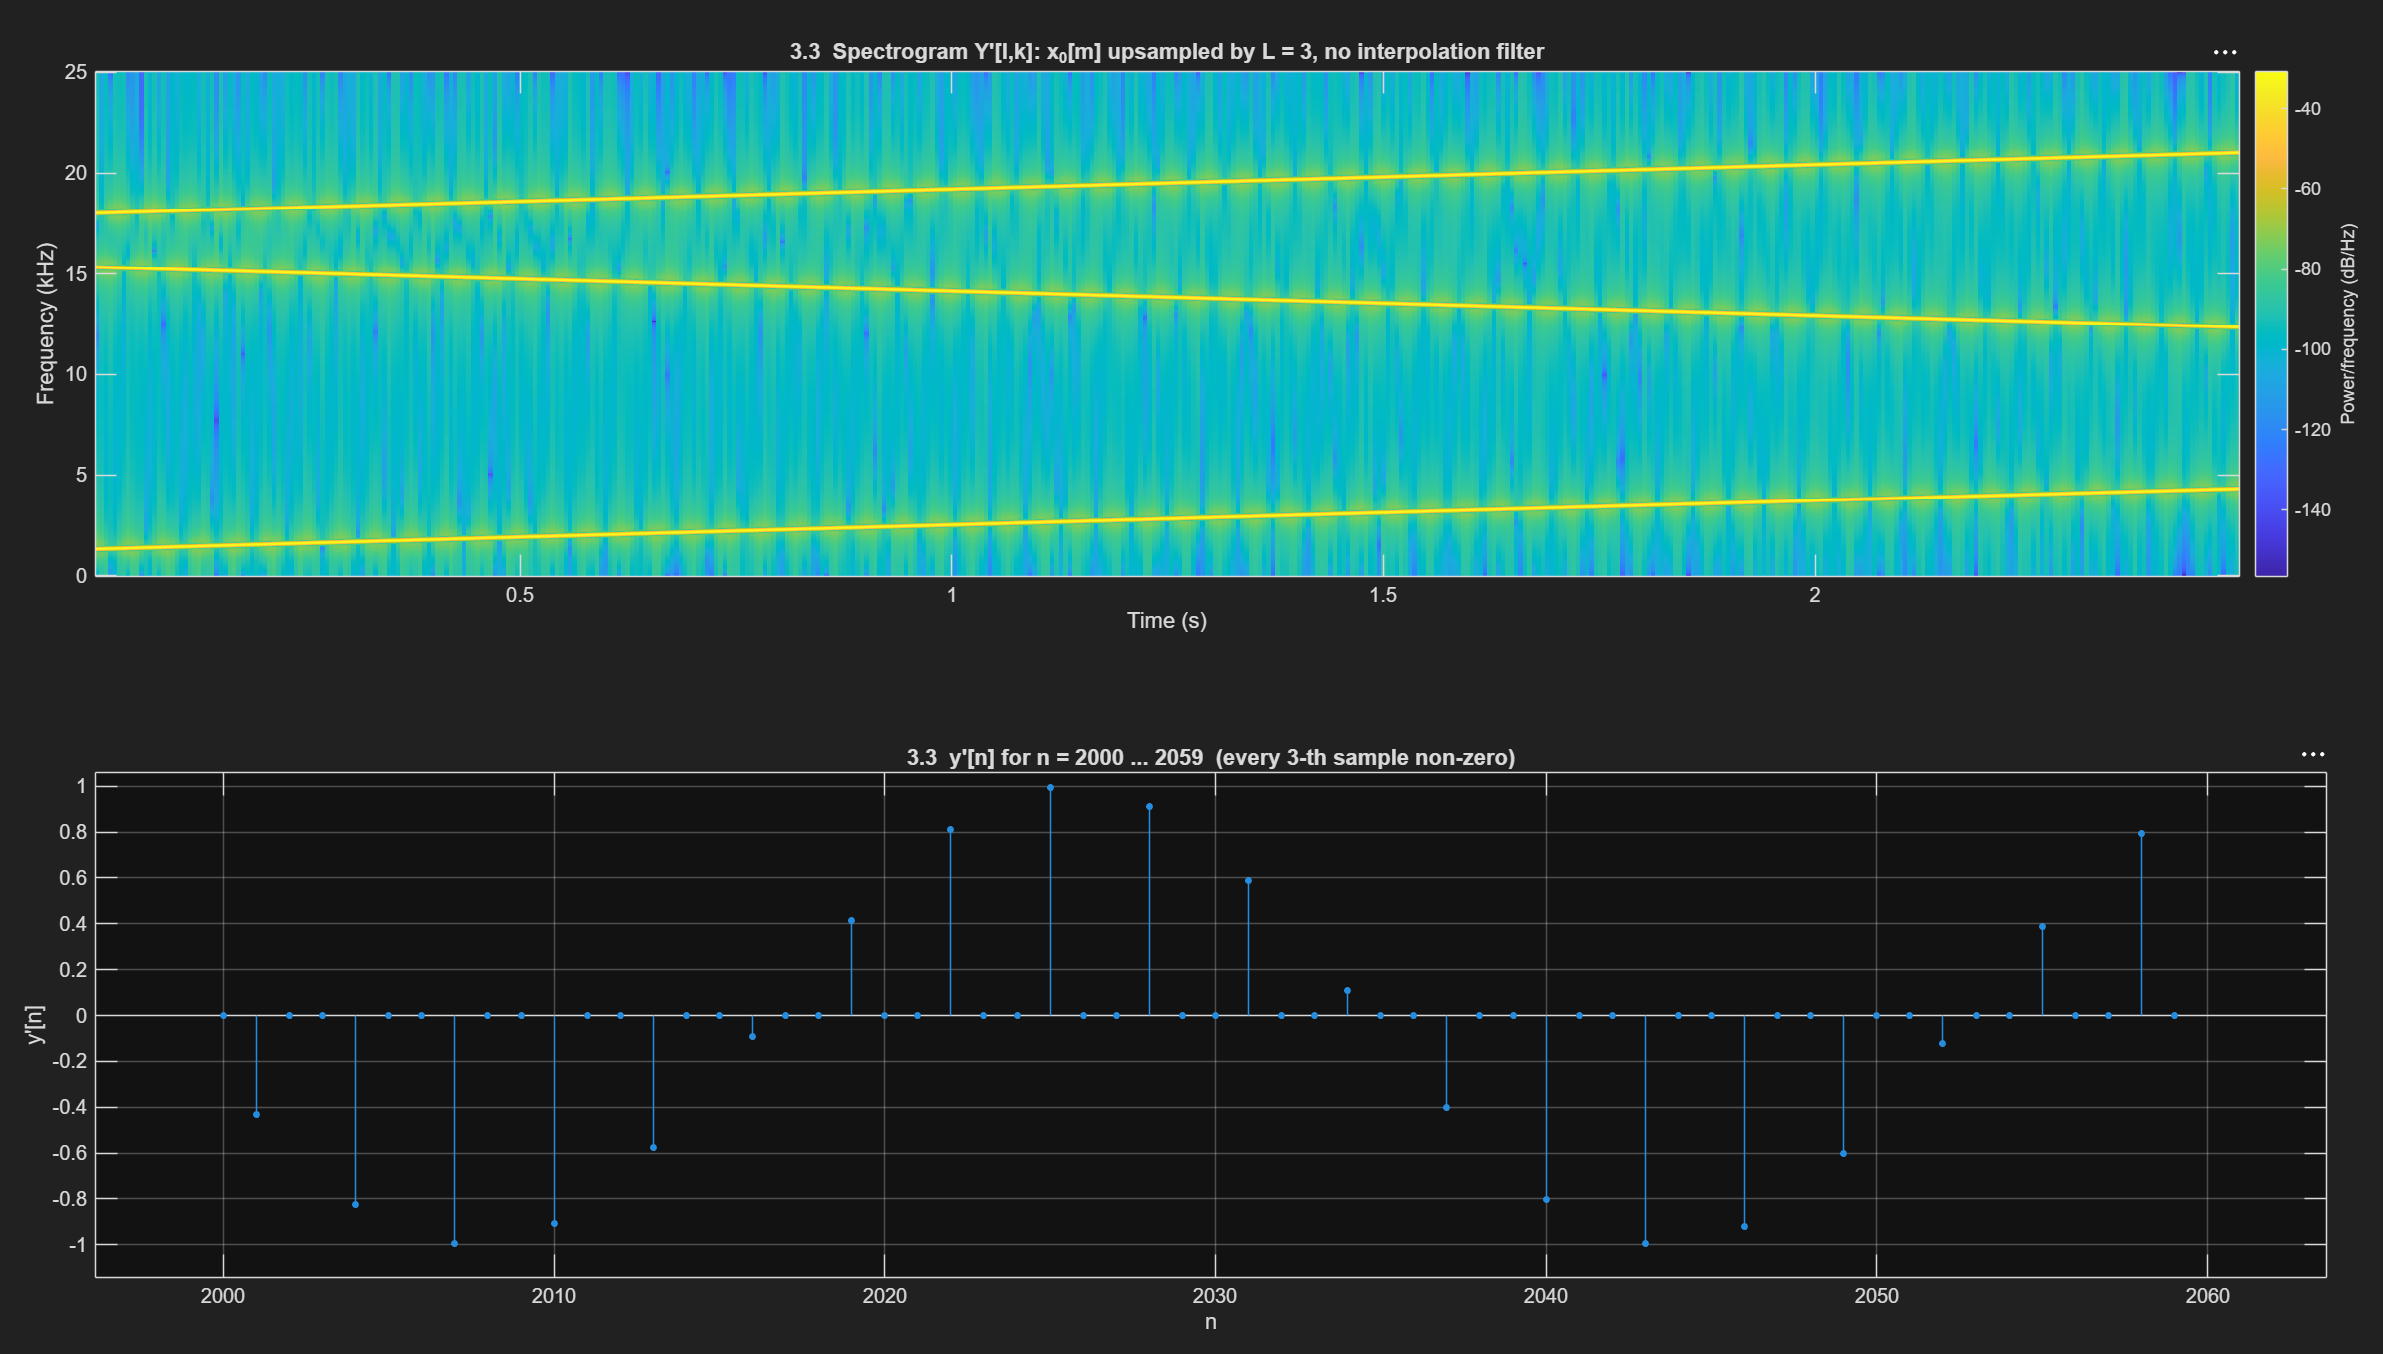
\includegraphics[width=1\linewidth]{ESP1_3,3}
		\caption{Upsampler output $y'[n]$ ($L = 3$, no interpolation filter): spectrogram $Y'[l,k]$ (top) and stem plot for $n = 2000, \dots, 2059$ (bottom).}
		\label{fig:esp133}
	\end{figure}
	
	
	\noindent\textbf{Explanation.} Upsampling inserts $L - 1 = 2$ zeros between the samples of $x_0[m]$, which brings the signal back to the high sampling rate $f_s$ (see stem plot, every third sample is non-zero). The zeros do not restore the original signal: the spectrum of $x_0[m]$ is periodic with $f_s' = 16.67$\,kHz, and all periods within $0 \dots f_s/2$ become visible as images. The spectrogram therefore shows three chirps:
	\begin{itemize}
		\item baseband $f'$: 1.33\,kHz $\rightarrow$ 4.33\,kHz (rising), the chirp aliased by downsampling,
		\item first image $f_s' - f'$: 15.33\,kHz $\rightarrow$ 12.33\,kHz (falling, mirrored),
		\item second image $f_s' + f'$: 18\,kHz $\rightarrow$ 21\,kHz (rising), at the position of the original chirp.
	\end{itemize}
	All three components match the non-zero samples equally well, so they have the same level, each reduced to $1/L$ ($-9.5$\,dB).
	
	A bat sound of $f_{bat} = 18$\,kHz is first aliased to $18 - 16.67 \approx 1.33$\,kHz by downsampling. At the DAC output it is reproduced at 1.33\,kHz, 15.33\,kHz and 18\,kHz. It therefore appears at its original frequency of 18\,kHz, but attenuated and accompanied by two additional tones.
	
	\subsection{Applying an Interpolation Filter}
	
	\noindent\fbox{\parbox{\dimexpr\linewidth-2\fboxsep-2\fboxrule}{
			Add your results, including \textbf{Matlab code} and \textbf{figures}, to the preparation sheet.
			\textbf{Compare} the results from 3.3 and 3.4 and explain them.}}
	
	\medskip
	
	\begin{lstlisting}[style=matlab, caption={MATLAB code, Section 3.4}, label={lst:m34}]
		%% 3.4 Interpolation (anti-imaging) filter
		d_pass = 0.001;                  % pass-band ripple
		d_stop = 0.001;                  % stop-band ripple (-60 dB)
		
		% After upsampling the useful band of x_0 is 0 ... fs'/2 = fs/(2L).
		% The first image starts at fs' - fs'/2 = fs/(2L) -> the stop band must start there.
		f_stop = fs/(2*L);               % 8.333 kHz
		f_pass = f_stop - 1e3;           % 7.333 kHz, transition width 1 kHz
		
		[N_FIR, fo, mo, w] = firpmord([f_pass f_stop], [1 0], [d_pass d_stop], fs);
		N_firpmord = N_FIR;              % order estimated by firpmord
		
		% firpmord only ESTIMATES the order. The filter on the DSP uses 16-bit
		% coefficients, so check the quantised filter and increase N if necessary.
		while true
		b = L * firpm(N_FIR, fo, mo, w);     % gain L compensates the 1/L of zero insertion
		b = round(b*32768)/32768;            % Q15 quantisation exactly as on the DSP
		[H, fH] = freqz(b, 1, 2^15, fs);
		ripple  = max(abs(abs(H(fH <= f_pass))/L - 1));        % relative to gain L
		att_dB  = -20*log10(max(abs(H(fH >= f_stop)))/L);      % relative to gain L
		if ripple <= d_pass && att_dB >= -20*log10(d_stop)
		break;
		end
		N_FIR = N_FIR + 1;
		end
		fprintf('3.4: f_pass = %.3f kHz, f_stop = %.3f kHz\n', f_pass/1e3, f_stop/1e3);
		fprintf('     firpmord order %d, final order %d (%d coefficients)\n', ...
		N_firpmord, N_FIR, length(b));
		fprintf('     quantised filter: pass-band ripple %.5f, stop-band attenuation %.1f dB\n', ...
		ripple, att_dB);
		
		figure('Name', '3.4 Interpolation filter');
		plot(fH/1e3, 20*log10(abs(H)/L)); grid on; hold on;
		xline(f_pass/1e3, '--', 'f_{pass}'); xline(f_stop/1e3, '--', 'f_{stop}');
		yline(-60, ':', '-60 dB');
		xlim([0 fs/2e3]);                % 0 ... 25 kHz
		xticks(0:1:fs/2e3);              % tick every 1 kHz
		xlabel('f [kHz]'); ylabel('|H(f)| / L [dB]');
		title(sprintf('3.4  Interpolation filter, order %d, Q15 coefficients, gain L = %d', N_FIR, L));
		ylim([-100 5]);
		
		% apply the filter to the upsampler output
		y = filter(b, 1, yu);
		
		figure('Name', '3.4 Interpolation filter output y[n]');
		subplot(2,1,1);
		spectrogram(y, hamming(Nwin), Nover, Nfft, fs, 'yaxis');
		title('3.4  Spectrogram Y[l,k]: after interpolation filter');
		
		subplot(2,1,2);
		% longer section than in 3.1/3.3: the 1.333 kHz output has 37.5 samples per
		% period, 120 samples show about 3 periods
		n2_34 = n1 + 119;
		sel34 = (nu >= n1) & (nu <= n2_34);
		stem(nu(sel34), y(sel34), 'filled', 'MarkerSize', 3); grid on;
		xlabel('n'); ylabel('y[n]');
		title(sprintf('3.4  y[n] for n = %d ... %d  (group delay %.1f samples)', n1, n2_34, N_FIR/2));
	\end{lstlisting}
	
	\begin{figure}[H]
		\centering
		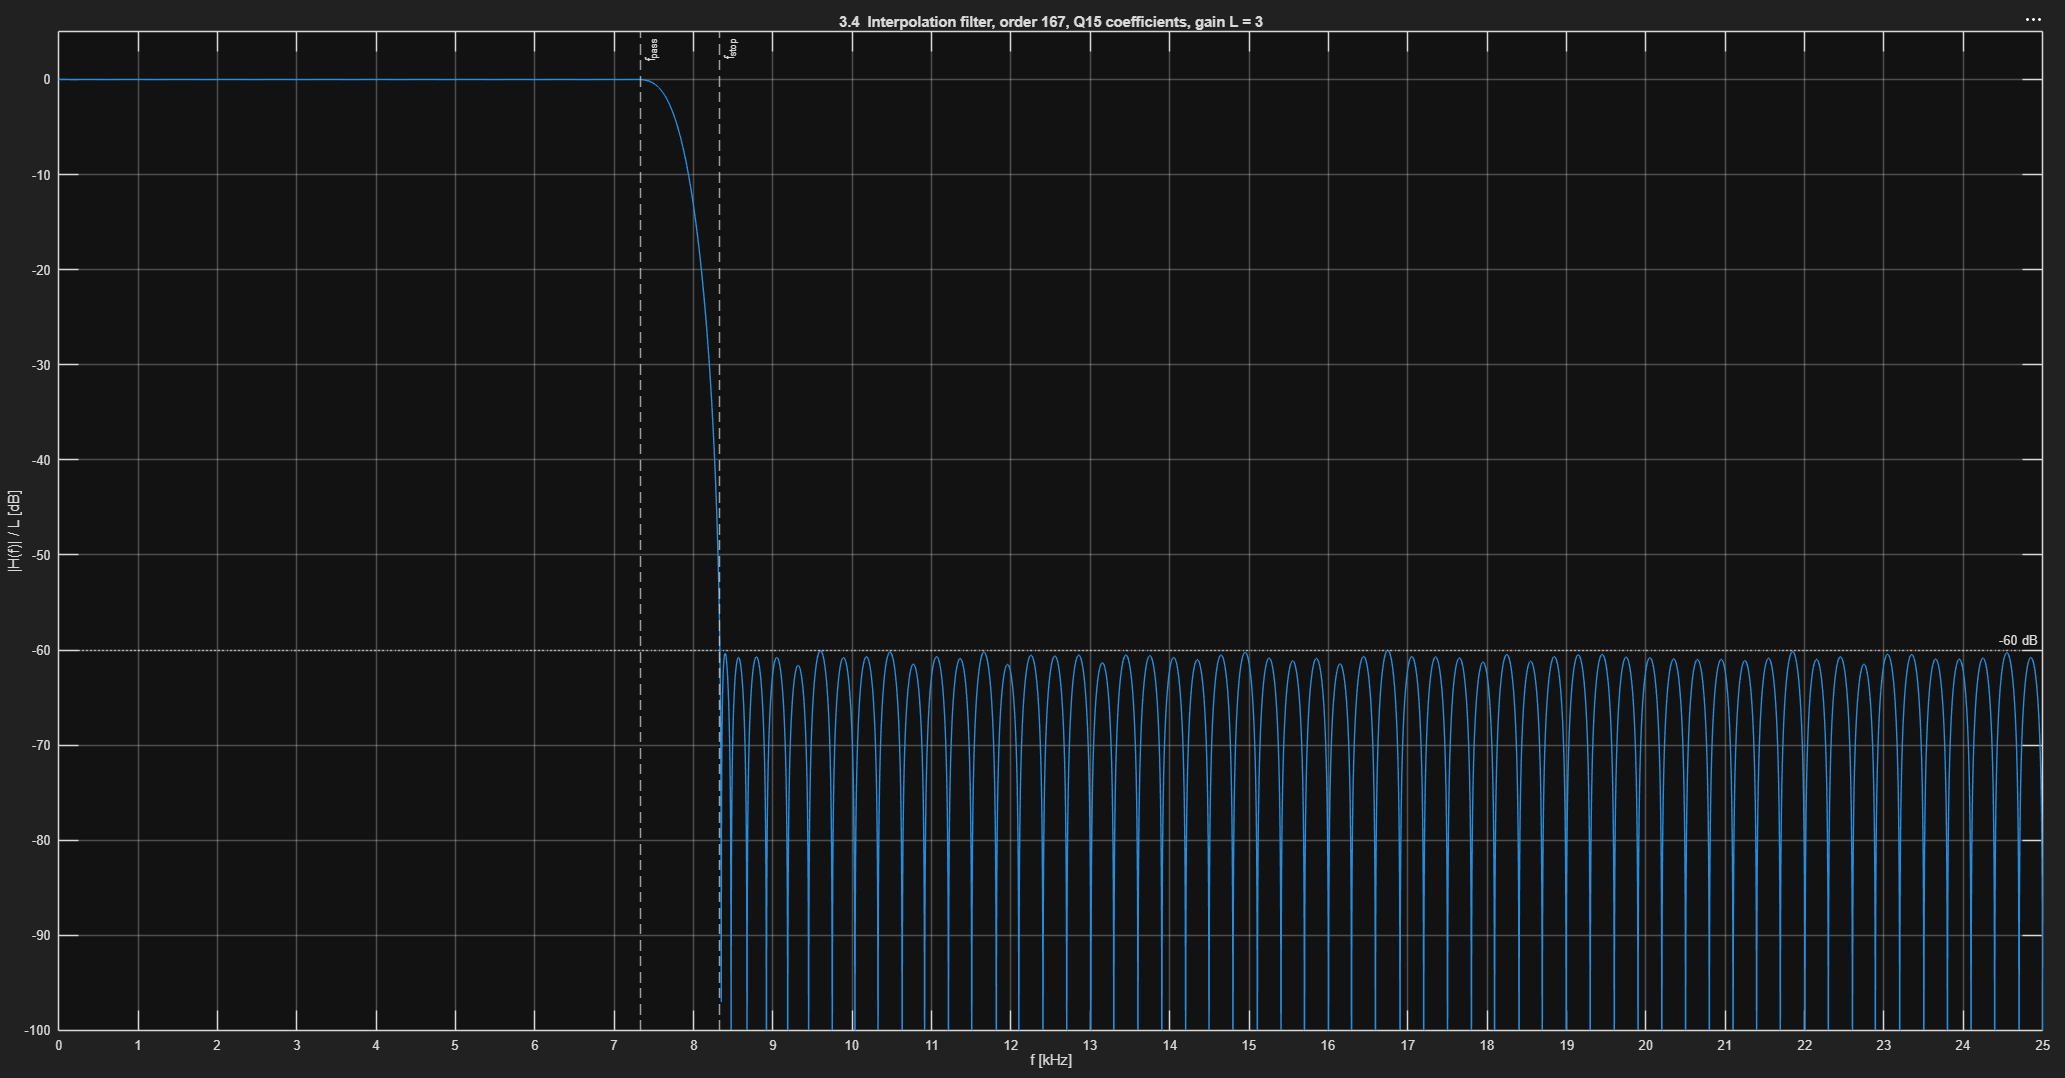
\includegraphics[width=1\linewidth]{ESP1_3,4_filter}
		\caption{FIR-Filter normalized frequency response }
		\label{fig:esp134filter}
	\end{figure}
	
	
	\begin{figure}[H]
		\centering
		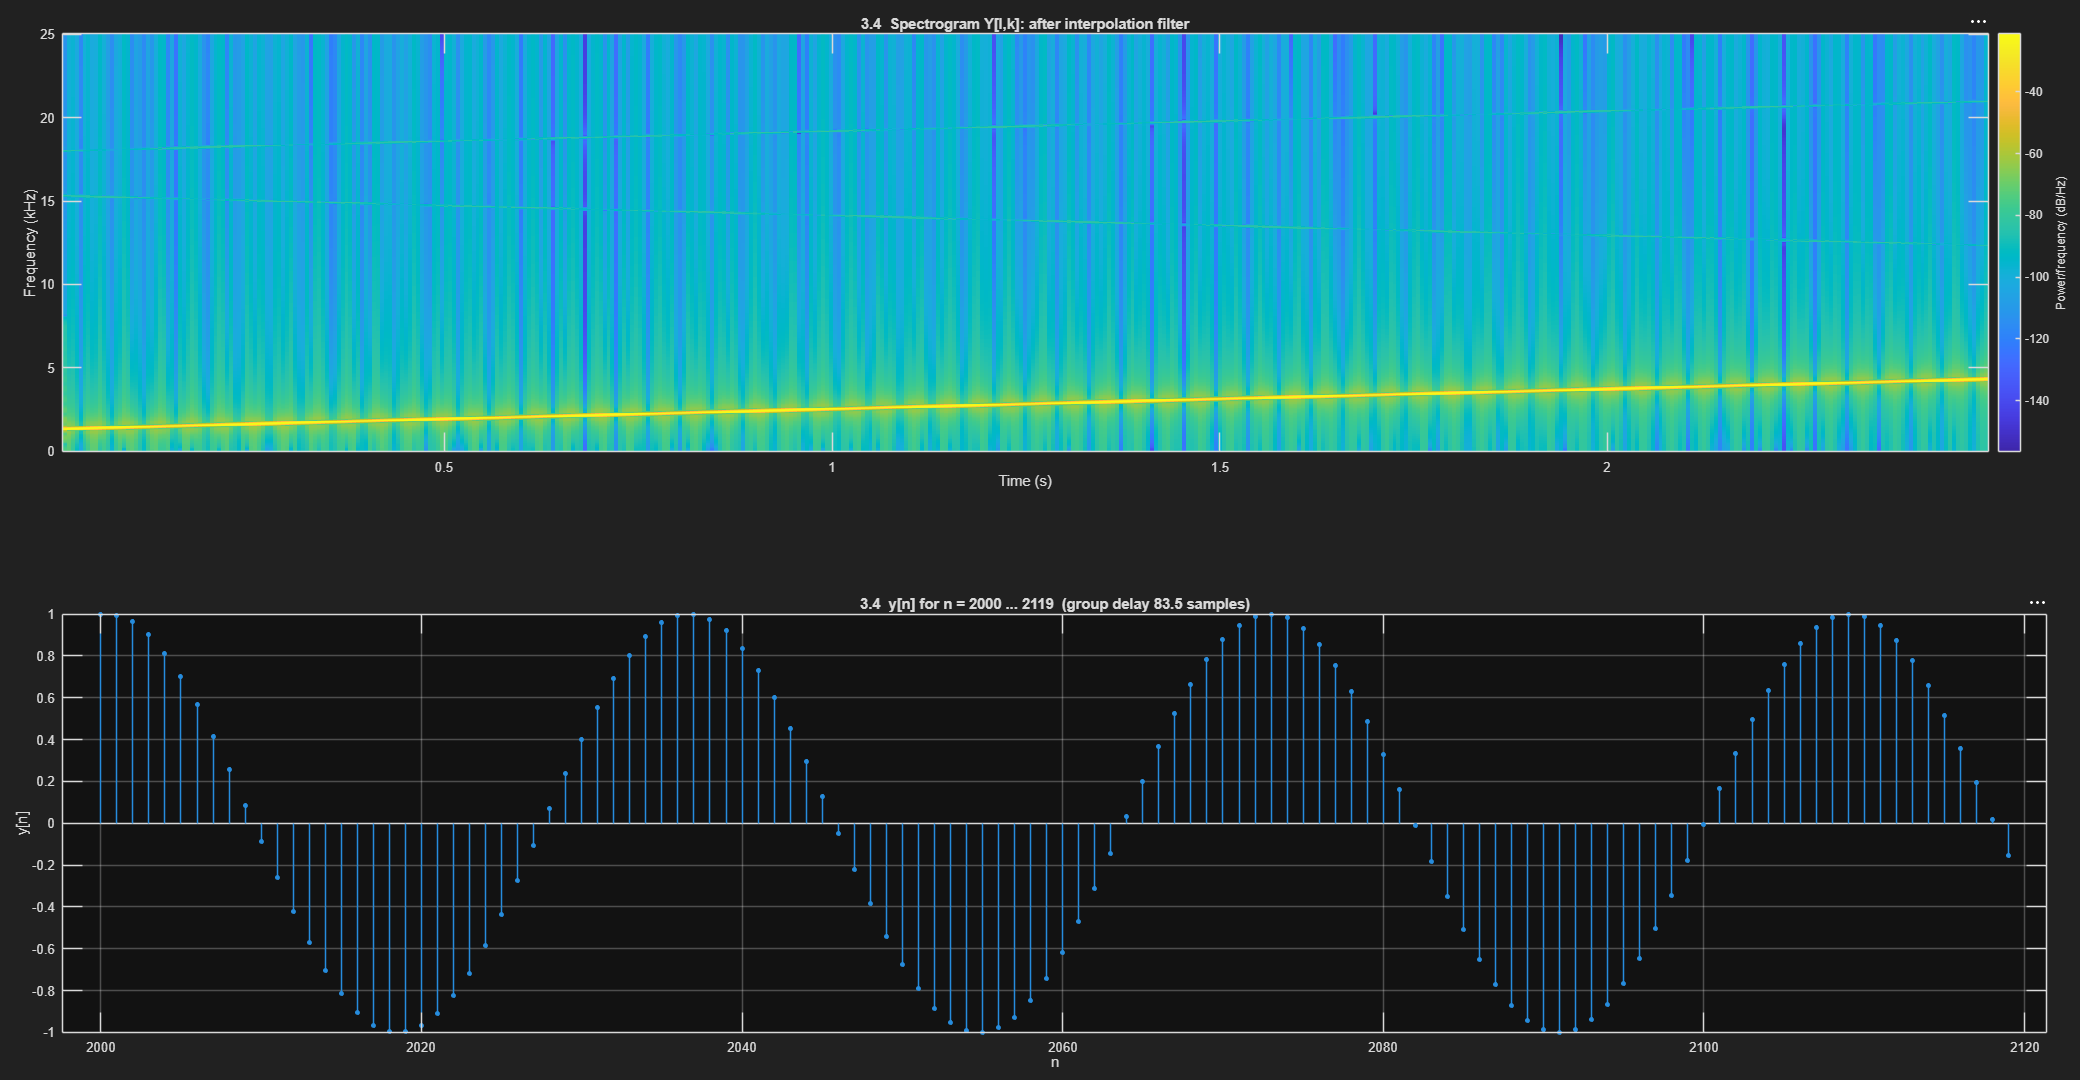
\includegraphics[width=1\linewidth]{ESP1_3,4}
		\caption{Interpolation filter output $y[n]$: spectrogram $Y[l,k]$ (top) and stem plot for $n = 2000, \dots, 2119$ (bottom).}
		\label{fig:esp134}
	\end{figure}
	
	\noindent\textbf{Explanation.} The interpolation filter is a low-pass filter with $f_{pass} = 7.33$\,kHz and $f_{stop} = f_s/(2L) = 8.33$\,kHz. It keeps the baseband chirp (1.33\,kHz $\rightarrow$ 4.33\,kHz) and suppresses both images (15.33\,kHz $\rightarrow$ 12.33\,kHz and 18\,kHz $\rightarrow$ 21\,kHz). The images are still faintly visible because a real FIR filter of finite order does not attenuate them completely: the design specification $\delta_{stop} = 0.001$ corresponds to 60\,dB, which matches the distance between the chirp and the remaining images in the spectrogram.
	
	Compared to 3.3, the zeros in the time signal have been filled. Each output sample of the FIR filter is a weighted sum of the last 168 input samples, which always contain non-zero values, so the filter interpolates the missing samples. In the frequency domain, only the baseband component remains, and a single sinusoid is non-zero at every sample. The stem plot therefore shows a smooth sine wave of about 1.33\,kHz. Its amplitude is 1 again, because the filter has the gain $L = 3$ that compensates the factor $1/L$ caused by zero insertion. 
	
	\subsection{Export Filter Coefficients to C}
	
	\noindent\fbox{\parbox{\dimexpr\linewidth-2\fboxsep-2\fboxrule}{
			\textbf{Generate} the header file for the filter coefficients of your interpolation filter and
			bring the file with you to the lab session. \textbf{How many coefficients} does your FIR filter
			have? Which is the \textbf{largest and which the smallest} value? Do these values \textbf{fit into
				16-bit format}? \textbf{Explain}.}}
	
	\medskip
	
	\begin{lstlisting}[style=matlab, caption={MATLAB code, Section 3.5}, label={lst:m35}]
		%% 3.5 Export filter coefficients to a C header file
		coeff_q15 = round(b*32768);                 % integer values written by write_coeff
		if any(coeff_q15 > 32767) || any(coeff_q15 < -32768)
		error('Coefficient outside 16-bit range -> reduce gain or rescale!');
		end
		
		filename = 'interp_filter_L3.h';
		file_ID  = fopen(filename, 'w');
		fprintf(file_ID, '//------------------------------------------- \n');
		fprintf(file_ID, '// designed with -- ESP_Lab1_Prep_ESPL01.m -- \n');
		fprintf(file_ID, ['// ', date, '\n']);
		fprintf(file_ID, '// interpolation filter, L = %d, gain = L\n', L);
		fprintf(file_ID, '// Fs = %8.2f\n', fs);
		fprintf(file_ID, '// fpass = %8.2f\n', f_pass);
		fprintf(file_ID, '// fstop = %8.2f\n', f_stop);
		fprintf(file_ID, '// delta_pass = %6.4f\n', d_pass);
		fprintf(file_ID, '// delta_stop = %6.4f (%.0f dB)\n', d_stop, 20*log10(d_stop));
		fprintf(file_ID, '// N_FIR = %d (firpmord estimate %d)\n', N_FIR, N_firpmord);
		fprintf(file_ID, '//------------------------------------------- \n');
		fprintf(file_ID, '#define N_DELAYS_INTERP %d\n', length(b));
		fprintf(file_ID, 'short H_interp_delays[N_DELAYS_INTERP]; \n');
		write_coeff(file_ID, 'b_interp', b, length(b));
		fclose(file_ID);
		
		fprintf('3.5: header %s written\n', filename);
		fprintf('     number of coefficients: %d\n', length(coeff_q15));
		fprintf('     largest  value: %6d  (%.4f)\n', max(coeff_q15), max(coeff_q15)/32768);
		fprintf('     smallest value: %6d  (%.4f)\n', min(coeff_q15), min(coeff_q15)/32768);
		fprintf('     sum of coefficients (DC gain): %.4f\n', sum(b));
	\end{lstlisting}
	
	\begin{lstlisting}[style=ccode,caption={generated C-Header with write\_coeff.m }, label={lst:C-headerfile3.5}]
		//------------------------------------------- 
		// designed with -- ESP_Lab1_Prep_ESPL01.m -- 
		// 31-Oct-2026
		// interpolation filter, L = 3, gain = L
		// Fs = 50000.00
		// fpass =  7333.33
		// fstop =  8333.33
		// delta_pass = 0.0010
		// delta_stop = 0.0010 (-60 dB)
		// N_FIR = 167 (firpmord estimate 163)
		//------------------------------------------- 
		#define N_DELAYS_INTERP 168
		short H_interp_delays[N_DELAYS_INTERP]; 
		short b_interp[168]={
			28,    -36,    -37,    -24,      5,     30,
			28,     -4,    -39,    -43,     -5,     45,
			60,     19,    -48,    -80,    -40,     45,
			100,     66,    -36,   -119,   -100,     19,
			136,    139,     10,   -146,   -183,    -50,
			148,    229,    103,   -137,   -276,   -170,
			110,    318,    249,    -63,   -352,   -340,
			-6,    372,    440,    100,   -372,   -544,
			-222,    345,    649,    374,   -285,   -748,
			-556,    183,    833,    770,    -30,   -896,
			-1016,   -187,    924,   1298,    483,   -904,
			-1621,   -887,    813,   2001,   1448,   -615,
			-2473,  -2275,    233,   3134,   3653,    548,
			-4303,  -6636,  -2665,   7860,  20754,  29572,
			29572,  20754,   7860,  -2665,  -6636,  -4303,
			548,   3653,   3134,    233,  -2275,  -2473,
			-615,   1448,   2001,    813,   -887,  -1621,
			-904,    483,   1298,    924,   -187,  -1016,
			-896,    -30,    770,    833,    183,   -556,
			-748,   -285,    374,    649,    345,   -222,
			-544,   -372,    100,    440,    372,     -6,
			-340,   -352,    -63,    249,    318,    110,
			-170,   -276,   -137,    103,    229,    148,
			-50,   -183,   -146,     10,    139,    136,
			19,   -100,   -119,    -36,     66,    100,
			45,    -40,    -80,    -48,     19,     60,
			45,     -5,    -43,    -39,     -4,     28,
			30,      5,    -24,    -37,    -36,     28,
		};
	\end{lstlisting}
	
	
	\begin{lstlisting}[style=matlab, caption={MATLAB command window output, Section 3.5}, label={lst:out35}]
		3.5: header interp_filter_L3.h written
		number of coefficients: 168
		largest  value:  29572  (0.9025)
		smallest value:  -6636  (-0.2025)
	\end{lstlisting}
	
	\noindent\textbf{Explanation.} The FIR filter has 168 coefficients (order 167). The largest coefficient is 29572 (0.9025), the smallest is $-6636$ ($-0.2025$). The coefficients are symmetric, as expected for a linear-phase FIR filter.\texttt{write\_coeff} converts the floating-point coefficients into the 16-bit Q15 format: each coefficient is multiplied by $2^{15} = 32768$ and rounded to an integer,

	A 16-bit signed integer covers the range $-32768 \dots 32767$, which corresponds to $-1 \le h < 1$. Both the largest value $0.9025$ and the smallest value $-0.2025$ lie within this range, so all coefficients fit into the 16-bit format, even though the filter contains the gain $L = 3$. On the DSP, the products of samples and coefficients are summed in a 32-bit accumulator and shifted back by 15 bits (\texttt{shft = 15}) to obtain a 16-bit output sample.
	
	% ------------------------------------------------------------------
	\subsection{C Program with Interrupt Handlers}
	
	\noindent\fbox{\parbox{\dimexpr\linewidth-2\fboxsep-2\fboxrule}{
			\textbf{Extend the code} for $M$ and $L$ values given in Table~1 for your ESPL group. The
			\textbf{polyphases} $x_{\lambda m}$ specified in Table~1 should be \textbf{fed to the respective
				DAC outputs}. \textbf{Why} is \texttt{g\_PolyWUpdate} necessary? \textbf{Add your C code} to the
			preparation sheet.}}
	
	\medskip
	\newpage
	\begin{lstlisting}[style=ccode, caption={C code for $M = L = 3$ in the DSP program (DAC CH0: $\lambda = 0$, CH1: $\lambda = 2$), Section 3.6}, label={lst:c36}]
		// main_adda_simple_Lab.c (Appendix A.2, "Getting Started with UniDAQ2"):
#include <stdio.h>

#define M 3    // downsampling factor
#define L 3    // upsampling factor
#define LEN 30
#define ADC0 0
#define ADC1 1

// Global variable declaration
short int g_PolyW[M]={0,0}; // downsampled polyphase values
short int g_PolyWUpdate=0;   // last polyphase updated
short int g_i16AdcData[2]={0,0};  // 2 x 16 bit data of ADC input channels
short int g_i16DacData[2]={0,0};; // 2 x 16 bit data of DAC output  channels

short int g_SamplesX[30] = {
	1,2,3,4,5,6,7,8,9,10,
	11,12,13,14,15,16,17,18,19,20,
	21,22,23,24,25,26,27,28,29,30
}; // input values
short int g_SampleXIdx = 0; // index input samples

// decimation
void adcInt(void) {
	static short lambda = 0;
	// read values from ADC
	g_i16AdcData[ADC0] = g_SamplesX[g_SampleXIdx]; // next ADC sample
	g_i16AdcData[ADC1] = 0;                        // 2nd channel not used
	
	// create polyphase signals, low sampling rate 
	switch (lambda) {
		case 0:
		g_PolyW[0] = g_i16AdcData[ADC0];
		g_PolyWUpdate = 0;
		break;
		case 1:
		g_PolyW[1] = g_i16AdcData[ADC0];
		g_PolyWUpdate = 1;
		break;
		case 2: 
		g_PolyW[2] = g_i16AdcData[ADC0];
		g_PolyWUpdate = 2;
		break;
		default:
		break;
	}
	
	lambda = (lambda + 1) % M;
}

void dacInt(void) {
	// write values to DAC, high sampling rate
	switch (g_PolyWUpdate) {
		case 0:
		g_i16DacData[0] = g_PolyW[0];
		g_i16DacData[1] = 0;
		break;
		case 1:
		g_i16DacData[0] = 0; // both DAC output should be set to zero during polyphase = 1
		g_i16DacData[1] = 0;
		break;
		case 2: 
		g_i16DacData[0] = 0;
		g_i16DacData[1] = g_PolyW[2];
		break;
		default:
		break;
	}
	// add interpolation filtering here
}

int main(void) {
	short int g_SamplesY[2][LEN]; // output values
	
	for (g_SampleXIdx = 0; g_SampleXIdx < LEN; g_SampleXIdx++) {
		dacInt(); // "call" of interrupt handler
		adcInt(); // "call" of interrupt handler
		
		// output values after ADC + DAC interrupt
		printf("g_PolyW[0]:%2d  g_PolyW[2]:%2d\n", g_PolyW[0], g_PolyW[2]); 
		g_SamplesY[0][g_SampleXIdx] = g_i16DacData[0];
		g_SamplesY[1][g_SampleXIdx] = g_i16DacData[1];
	}
	
	// assemble polyphase signals y_0[n], y_1[1]
	printf("g_SamplesY[0]: ");
	for (g_SampleXIdx = 0; g_SampleXIdx < LEN; g_SampleXIdx++) {
		printf("%d ", g_SamplesY[0][g_SampleXIdx]);
	}
	printf("\n");
	
	printf("g_SamplesY[1]: ");
	for (g_SampleXIdx = 0; g_SampleXIdx < LEN; g_SampleXIdx++) {
		printf("%d ", g_SamplesY[1][g_SampleXIdx]);
	}
	printf("\n");
	
	return 0;
}
	\end{lstlisting}
	
	\begin{lstlisting}[style=ccode, numbers=none, basicstyle=\ttfamily\tiny, columns=fixed, breaklines=false, caption={Simulated output of \texttt{adcInt()}/\texttt{dacInt()} for the input values 1 to 30 and both interrupt orders, Section 3.6}, label={lst:out36}]
g_PolyW[0]: 1  g_PolyW[2]: 0
g_PolyW[0]: 1  g_PolyW[2]: 0
g_PolyW[0]: 1  g_PolyW[2]: 3
g_PolyW[0]: 4  g_PolyW[2]: 3
g_PolyW[0]: 4  g_PolyW[2]: 3
g_PolyW[0]: 4  g_PolyW[2]: 6
g_PolyW[0]: 7  g_PolyW[2]: 6
g_PolyW[0]: 7  g_PolyW[2]: 6
g_PolyW[0]: 7  g_PolyW[2]: 9
g_PolyW[0]:10  g_PolyW[2]: 9
g_PolyW[0]:10  g_PolyW[2]: 9
g_PolyW[0]:10  g_PolyW[2]:12
g_PolyW[0]:13  g_PolyW[2]:12
g_PolyW[0]:13  g_PolyW[2]:12
g_PolyW[0]:13  g_PolyW[2]:15
g_PolyW[0]:16  g_PolyW[2]:15
g_PolyW[0]:16  g_PolyW[2]:15
g_PolyW[0]:16  g_PolyW[2]:18
g_PolyW[0]:19  g_PolyW[2]:18
g_PolyW[0]:19  g_PolyW[2]:18
g_PolyW[0]:19  g_PolyW[2]:21
g_PolyW[0]:22  g_PolyW[2]:21
g_PolyW[0]:22  g_PolyW[2]:21
g_PolyW[0]:22  g_PolyW[2]:24
g_PolyW[0]:25  g_PolyW[2]:24
g_PolyW[0]:25  g_PolyW[2]:24
g_PolyW[0]:25  g_PolyW[2]:27
g_PolyW[0]:28  g_PolyW[2]:27
g_PolyW[0]:28  g_PolyW[2]:27
g_PolyW[0]:28  g_PolyW[2]:30
g_SamplesY[0]: 0 1 0 0 4 0 0 7 0 0 10 0 0 13 0 0 16 0 0 19 0 0 22 0 0 25 0 0 28 0 
g_SamplesY[1]: 0 0 0 3 0 0 6 0 0 9 0 0 12 0 0 15 0 0 18 0 0 21 0 0 24 0 0 27 0 0 
	\end{lstlisting}
	
\noindent\textbf{Explanation.} The file \texttt{dec\_int\_standalone.c} for $M = L = 2$ was extended to $M = L = 3$ (Listing~\ref{lst:c36}):
\begin{itemize}
\item \texttt{M} and \texttt{L} are set to 3, and \texttt{g\_PolyW} has three elements.
\item \texttt{adcInt()} gets the additional \texttt{case 2}. The input samples are distributed cyclically to $\lambda = 0, 1, 2$, i.e.\ $x_\lambda[m] = x[3m + \lambda]$ (decimation by $M = 3$).
\item In \texttt{dacInt()}, \texttt{case 0} outputs $x_0[m]$ on CH0 and \texttt{case 2} outputs $x_2[m]$ on CH1. In all other DAC interrupts the channel receives a zero, so each polyphase value is followed by two zeros (upsampling by $L = 3$).
\end{itemize}
The output in Listing~\ref{lst:out36} confirms this: CH0 carries $1, 4, 7, \dots = x[0], x[3], x[6], \dots = x_0[m]$ and CH1 carries $3, 6, 9, \dots = x[2], x[5], x[8], \dots = x_2[m]$, each followed by two zeros. All values are delayed by one sample, because \texttt{main()} calls \texttt{dacInt()} before \texttt{adcInt()}, so the DAC outputs the value of the previous ADC interrupt. In the lab (Section 4.2), the bodies of \texttt{adcInt()} and \texttt{dacInt()} are inserted into the interrupt handlers of the \texttt{adda\_simple} project, with \texttt{g\_i16AdcData} and \texttt{g\_i16DacData} replaced by the ADC and DAC registers.

\medskip
\noindent\textbf{Why is \texttt{g\_PolyWUpdate} necessary?} \texttt{g\_PolyWUpdate} is the link between the two interrupt handlers: \texttt{adcInt()} writes which polyphase has just been updated, and \texttt{dacInt()} reads it to decide whether the current output sample is a polyphase value or an inserted zero. ADC and DAC interrupts are triggered independently, and their order cannot be predicted. A separate counter in \texttt{dacInt()} could therefore run out of phase with the ADC and output an old value or a value of the wrong polyphase. With \texttt{g\_PolyWUpdate}, the interpolation stays synchronised with the decimation
	
	\bigskip
	\noindent The preparation is complete. Congratulations!
	\textbf{Please submit the preparation sheet in Moodle before the lab session.}
	
\end{document}